\documentclass[a4paper]{article}
\usepackage{polski}
\usepackage[utf8]{inputenc}
\usepackage[margin=1in]{geometry}
\usepackage{listings}
\usepackage{graphicx}
\usepackage{amsmath}

\title{\textbf{Algorytmy Zaawansowane - kolorowanie $Delta(G)$ dokumentacja końcowa}}
\author{\textbf{Albert Sadowski, Piotr Stanek}\\
	Wydział Matematyki i Nauk Informacyjnych\\
	Politechnika Warszawska}

\begin{document}
	\maketitle

	\section{Instrukcja użytkownika}

	{\em Delta coloring} jest aplikacją konsolową realizującą algorytm kolorowania grafu o czasie wykonania ograniczonym przez {\em Delta(G)}.

	Aplikacja przyjmuje jako argument graf ścieżkę do pliku zawierającego graf zdefiniowany w formacie DOT. Plik wykonywalny {\em deltaColoring} do starndardowego wyjścia drukuje wynik realizacji algorytmu - graf w formacie DOT ze znacznikami odpowiadającymi za kolor poszczególnych wierzchołków grafu.

	Przykładowe uruchomienie programu:

	\begin{verbatim}

		deltaColoring /path/to/input.dot

	\end{verbatim}

	Skrypt {\em run.sh} uruchamia aplikację {\em deltaColoring} wraz z innymi programami odpowiadającymi za wygenerowania pliku PDF z pokolorowanym grafem wyjściowym - rezultatem programu. 

	Przykładowe uruchomienie skryptu:

	\begin{verbatim}

		run.sh /path/to/input.dot

	\end{verbatim}


	Skrypt korzysta z aplikacji {\em dot}, która rysuje graf podany w formacie DOT do formatu post script, oraz z aplikacji {\em ps2pdf}, która dla zadanego pliku w formacie post script generuje plik PDF. Skrypt automatycznie uruchamia program {\em evince} z wyjściowym grafem.

	Wyjściowy plik PDF ({\em graph.pdf}) zapisany jest w folderze {\em output} wraz z plikiem {\em err.log} odpowiadającym za zapis strumienia {\em stderr}.

	Przykładowe wejście - graf zdefiniowany w formacie DOT:

	\begin{verbatim}

		graph G {
			0;
			1;
			2;
			3;
			4;
			0--2 ;
			1--1 ;
			1--3 ;
			1--4 ;
			2--1 ;
			2--3 ;
			3--4 ;
			4--0 ;
			4--1 ;
		}
	

	\end{verbatim}

	Wywołanie programu {\em deltaColoring} z powyższym grafem zadanym jako argument:

	\begin{verbatim}

		graph G {
			node[shape="circle",style="filled"]
			col[label="Colors: 3",shape="box"];
			com[label="Components: 1",shape="box"];
			del[label="Delta: 6", shape="box"];
			0[fillcolor="#B88A00",label="0[0]"];
			1[fillcolor="#B88A00",label="1[0]"];
			2[fillcolor="#F5B800",label="2[1]"];
			3[fillcolor="#FF6633",label="3[2]"];
			4[fillcolor="#F5B800",label="4[1]"];
			0--2 [label="0"];
			1--1 [label="0"];
			1--3 [label="0"];
			1--4 [label="0"];
			2--1 [label="0"];
			2--3 [label="0"];
			3--4 [label="0"];
			4--0 [label="0"];
			4--1 [label="0"];
		}


	\end{verbatim}

	Wywołanie skryptu {\em run.sh} z powyższym grafem zadanym jako argument:
	
	\begin{center}

		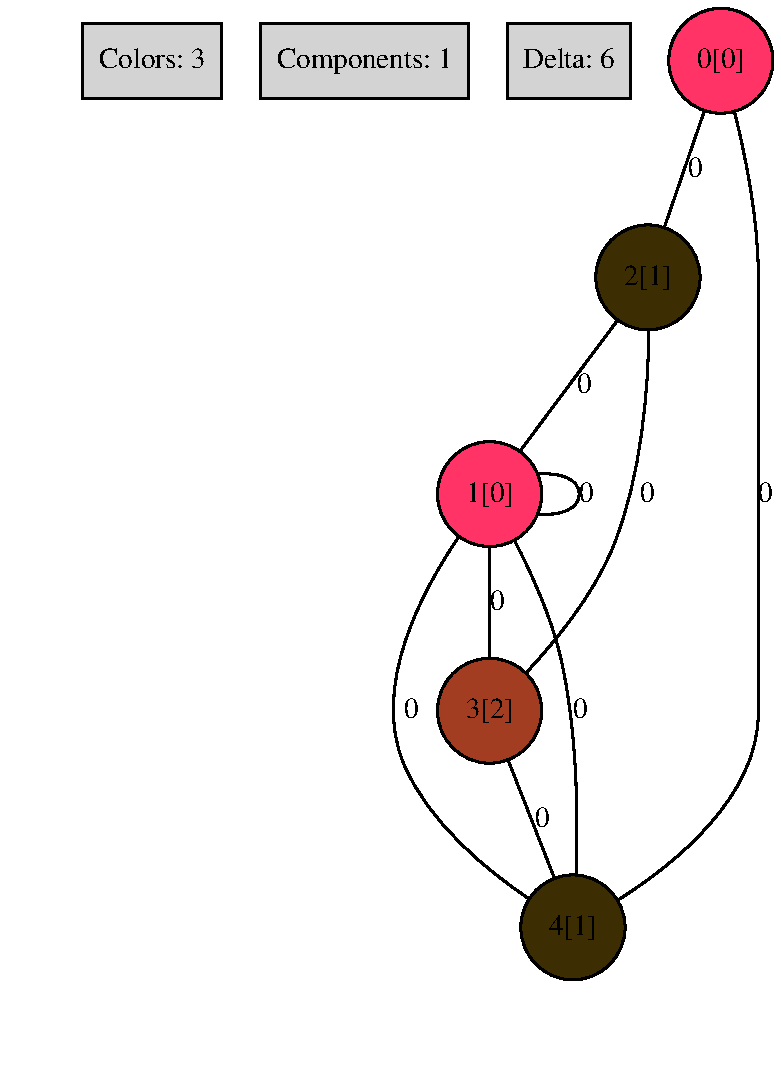
\includegraphics[height=12cm]{i1.pdf}

	\end{center}

	\section{Zmiany względem dokumentacji wstępnej}

		Dokumentacja wstępna nie przewidywała formy/sposobu działania aplikacji. Ze strony algorytmicznej nie wprowadzono zmian.

	\section{Wnioski}

	Do implementacji zastosowano bibliotekę Boost Graph Library (BGL). Implementacja podstawowych algorytmów teorii grafów (tj. przeszukanie w głąb, algorytm Dijkstry) dostarczona wraz z BGL została wykorzystana.

	\section{Podział prac}	

	\begin{itemize}

		\item {\em Albert Sadowski} - kolorowanie grafu spójnego, spajanie rozwiązań cząstkowych (dokumentacja wstępna + implementacja), dokumentacja finalna.

		\item {\em Piotr Stanek} - znajdowanie wierzchołków rozspajających (dokumentacja wstępna + implementacja), testy.

	\end{itemize}

\end{document}